% Created 2020-05-01 Fri 22:56
% Intended LaTeX compiler: pdflatex
\documentclass[a4paper, dvipdfmx, 10pt]{article}
\usepackage[utf8]{inputenc}
\usepackage[T1]{fontenc}
\usepackage{graphicx}
\usepackage{grffile}
\usepackage{longtable}
\usepackage{wrapfig}
\usepackage{rotating}
\usepackage[normalem]{ulem}
\usepackage{amsmath}
\usepackage{textcomp}
\usepackage{amssymb}
\usepackage{capt-of}
\usepackage{hyperref}
\usepackage{minted}
\usepackage{amsmath, amssymb, bm}
\usepackage{graphics}
\usepackage{color}
\usepackage{times}
\usepackage{longtable}
\usepackage{minted}
\usepackage{fancyvrb}
\usepackage{indentfirst}
\usepackage{pxjahyper}
\usepackage[utf8]{inputenc}
\usepackage[backend=biber, bibencoding=utf8]{biblatex}
\usepackage[top=20truemm, bottom=25truemm, left=25truemm, right=25truemm]{geometry}
\hypersetup{colorlinks=false, pdfborder={0 0 0}}
\usepackage{ascmac}
\usepackage{algorithm}
\usepackage{algorithmic}
\addbibresource{./qareport.bib}
\author{MokkeMeguru}
\date{\textit{<2019-04-24 Wed>}}
\title{GANs x テキスト生成の SOTA LeakGAN を読む}
\begin{document}

\maketitle
\tableofcontents

\section{導入}
\label{sec:org51e9dc4}
\href{https://arxiv.org/pdf/1709.08624v2.pdf}{LeakGAN} [1] というのは 2018 年に AAAI に掲載されたテキスト生成に関する論文です. GANs というと 画像生成として有名ですが、こいつをテキスト生成としてやっていこうという流れが当時からあり, SeqGAN あたりの流れから来ています. こいつは実はめちゃめちゃ色々な技術がもりもりしていて、具体的には CNN / RNN / Reinforest Learning 当たりの技術が全部入ってます. なのでこいつが理解できるというのはある程度広範の機械学習の技術が身についている、ということになります. 僕は Reinforest Learning 当たりは門外漢なので読むのがかなり辛かったです.

[1]: Long Text Generation via Adversarial Training with Leaked Information
\section{テキスト生成って何?}
\label{sec:orga934a04}
テキスト生成とは大まかに次の3種類に分かれています.
\begin{enumerate}
\item 何からの単語を皮切りに, それ以降の文を続けて生成していくもの. (GPT Series)
\item 何らかのランダムな値を入力して, 何らかの文を生成するもの. (GANs Series / AutoEncoder Series)
\end{enumerate}

どっちが良いのかとかではなく、分野の違いなのでこの辺りを気にしてはいけません。但し日本のイケイケNLP界隈的には前者の方が人気みたいです。(BERTとGPT Series が構造的に似ている.\\
LeakGAN は 2 の方の手法で直感的にはなんかよくわからい箱 (モデル) をえいやっと叩くと, なんかよくわからないけどそれっぽい文がポンッと出てくる、そんなイメージで大丈夫です.\\

正確には 2. には2種類存在しており, 1つは文を何らかの空間へ写像、その逆を行うことを目的とする AutoEncoder 形式, 何らかの空間からポンッと文を取り出すことを目的とした GANs 形式の2つです. LeakGAN は GANs 形式であり, 何らかの文をエイヤッとベクトル化するようなことは出来ません. まあ、GANs は全てなので, GANs 形式で研究しておけば何でも良いんですよ. (適当)
\section{どんな性能が出たの?}
\label{sec:org133c49c}
\subsection{概要}
\label{sec:org3a63286}
こんな感じの文がポンッと出てきました.

\begin{itemize}
\item A man sitting in front of a microphone with his dog sitting on his shoulder.
マイクの前で犬を方に乗せて座っている男
\item A young man is holding a bottle of wine in his hand.
手にワインボトルを持った若い男
\end{itemize}

つまるところまあ、論文上の結果を観る限り定性的にはそれなりに良い文章が出てきた、ということです.
\subsection{細かい話}
\label{sec:org5be6489}
実はこの分野、評価手法があまり定まっておらず、最近ですと Texygen [2] なんかでまとめられている NLL-oracle / NLL-test / BLEU / Self-BLEU / EmbSim, 更に ARAE で提案されている PPL / reverse PPL [3] 辺りが有力な候補として上がっていますが、それでも議論が尽きないといった有様です. (最悪どれか1つ勝っていれば論文にはなるんじゃないっすかね)\\

そんな中で LeakGANs が用いている評価手法は BLEU Score と人手による A/B テストですが, これだと実は評価手法としては \textbf{ゴミ} なので、別の論文 Texygen の方を参照する必要があります [4] .\\

細かい話は別の記事で書きますが, 直感的な説明を書いておきます.

[2]: \url{https://github.com/geek-ai/Texygen}

[3]: \url{https://pdfs.semanticscholar.org/15de/8ec5191e48cc111f7f8f31d35f280e4aadec.pdf}

[4]: \url{https://arxiv.org/pdf/1802.01886.pdf}

\subsubsection{NLL-oracle, NLL-test}
\label{sec:orge269dd3}
一般に自然言語のモデリングは, 自然言語という後半な広範囲なスケールのために, 正確な評価値を求めることが難しいことが知られています. そのため、自然言語ではなく、何らかの規則に基づいた系列データを生成することが考えられます. 本手法ではその規則生成に RNN を用いたモデルが提案されており、具体的なシード値とともに公開されています(tensorflow==1.5 です. つまりめちゃめちゃ面倒). Texygen や 先行研究の SeqGAN などは, この手法を用いることで定量的な評価が出来たもの、としました.\\
NLL-oracle の oracle こそが その生成モデルであり, NLL-test は, NLL-oracle の応用です. なぜ必要なのかは別の機会に詳しく説明しますが、簡単に言ってしまえばGANs の一大課題である mode collapse の回避のためです.\\
なお NLL-oracle , NLL-test は lower is better の指標です.\\
以下が結果になります. LeakGANs が NLL-oracle 敵にはそこそこでも, NLL-test 的に低い値を出していることが確認できると思います.

\begin{center}
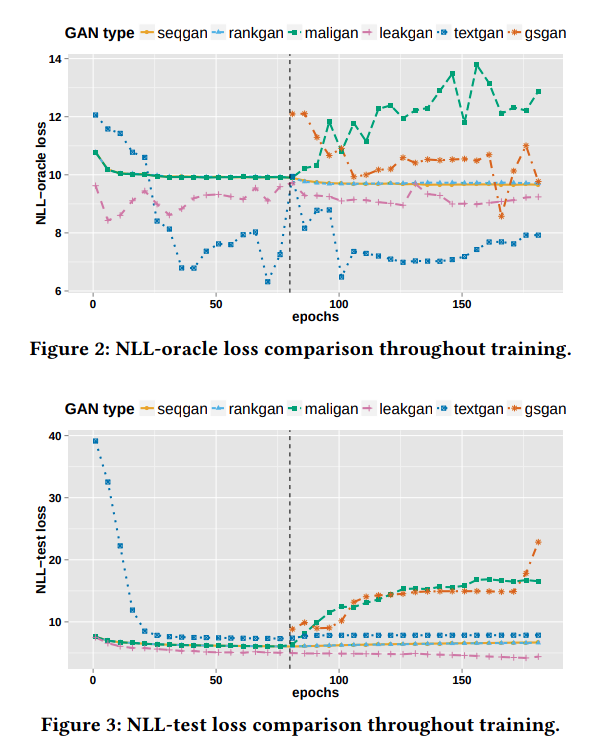
\includegraphics[width=10cm]{./img/oracle.png}
\end{center}

\subsubsection{BLEU Score}
\label{sec:orgbe61fd0}
BLEU Score は機械翻訳の分野で広く使われる手法であり, その分野では生成された文と人手で翻訳した文の一致度を n-gram というものを使って評価します. n-gram 一致度とはすなわち 特定の短い単語列の繋がりが合致しているかを測る指標で, 一般的な構文規則をモデル化出来ているかが判断できます.\\
言語モデルの評価としての BLEU Score は式こそ同じですが全く異なるものを求めることで, 非常に混乱する指標となっています. (ついでにいうとこの指標は *不適切* であるとされています)\\
言語モデルの評価時に用いられる BLEU Score は ランダムに生成された文とテストデータセット (学習に使わなかった自然言語の文) との n-gram 一致度を評価します. これによって例えば "at the" のような特定の言語規則を捉えていることを確認することが出来ます. この評価手法の弱点は GANs  の mode collapse に有利であるという点です(特定のそれっぽい文しか生成されないモデルでも、本スコアは非常に良い値を示します). LeakGANのオリジナルは BLEU Score で評価していましたが, まあ、GANs なので多少はね、というわけです.
\subsubsection{Self-BLEU Score}
\label{sec:org36252a6}
Self-BLEU Score は言語モデルにおける BLEU Score を改善 / 補足させるための指標です. これは 生成された文のうちの1文とそれ以外の生成文との n-gram 一致度を評価します。これによって似たような文が生成されてしまったことを定量的に評価することが出来ます。このためこの手法は "一致度" と言っておきなら, 低いほど良いスコアとみなします。
\section{GANs って何?}
\label{sec:org62edd51}
\section{強化学習って何?}
\label{sec:org4bc3a44}
\section{LeakGANs の構造ってどんな感じ?}
\label{sec:org0f18131}
\section{実装はどこ?再現実験したいんだけど}
\label{sec:org38cfcf8}
\section{読んだ感想とか}
\label{sec:org2ad0298}
\end{document}
